%  This LaTeX template is based on T.J. Hitchman's work which is itself based on Dana Ernst's template.
%
% --------------------------------------------------------------
% Skip this stuff, and head down to where it says "Start here"
% --------------------------------------------------------------

\documentclass[12pt]{article}

\usepackage[margin=1in]{geometry}
\usepackage{amsmath,amsthm,amssymb}
\usepackage{graphicx}
\usepackage[UTF8]{ctex}
\usepackage{listings}
\usepackage{cite}
\usepackage{subfigure}
%the following is used for the pseudo-code
\makeatletter
\newif\if@restonecol
\makeatother
\let\algorithm\relax
\let\endalgorithm\relax
\usepackage[linesnumbered,ruled,vlined]{algorithm2e} %[ruled,vlined]{
\usepackage{algpseudocode}
\usepackage{amsmath}
\renewcommand{\algorithmicrequire}{\textbf{Input:}}  % Use Input in the format of Algorithm
\renewcommand{\algorithmicensure}{\textbf{Output:}}  % Use Output in the format of Algorithm \begin{algorithm}


\begin{document}

% --------------------------------------------------------------
%
%                         Start here
%
% --------------------------------------------------------------

\title{三维计算机视觉的部分数学原理}
\author{王啸峰 from UCAS \& CASIA} % replace with your name

\maketitle
% 整体框架如图\ref{fig:framwork}:
% \begin{figure}[ht]
%     \centering
%     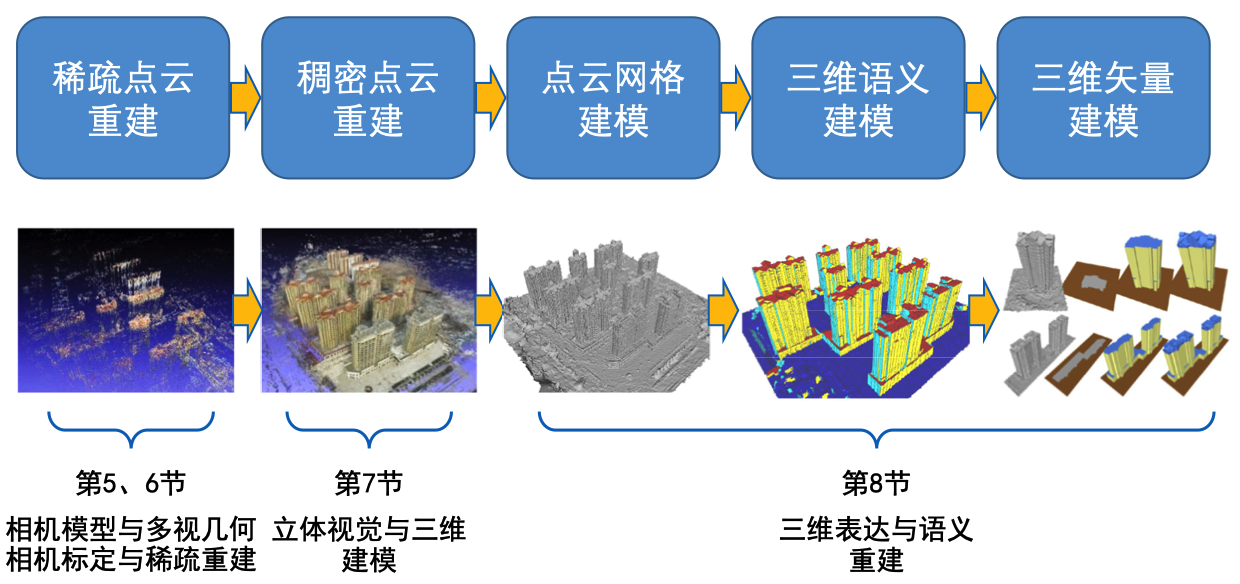
\includegraphics[scale=0.6]{./img/framwork.png}
%     \caption{框架图}
%     \label{fig:framwork}
% \end{figure}

\section{相机模型与多视几何}
% 先说故事:to be continue...
\subsection{欧式空间和射影空间}
先说故事:三维欧式空间可以很好的描述我们三维世界的“坐标点”,但是一旦涉及到二维图像,三维欧式坐标就不太好描述图像上像素点的位置了(因为图像上一个像素点对应的是三维空间中的
一条直线:光心和像素点连成的直线),所以需要射影空间来帮我们描述二维图像上的点和我们三维空间坐标的关系。以后我们就可以利用射影空间的性质(这部分比较复杂,本文只是粗略涉及)方便地计算出
我们想要的空间和图像上的几何关系。

\subsubsection{二维射影空间=变换尺度因子$\lambda \quad \times$齐次化的二维图像坐标=三维欧式空间过原点的直线+无穷远球面?}
小标题的含义只是粗略的理解这两个空间的变换关系(并且这个二维射影空间可能的表述应该是三维:多加了一维是$\lambda$),下面给出数学表达:

我们看下面图片,$[x,y]^T$是二维图像平面上的坐标,$[X,Y,Z]$是欧式空间中的三维坐标,$f$是焦距,根据红绿两个相似三角形,
我们可以得到:
\begin{equation}
    \lambda\left[\begin{array}{l}
        x \\
        y \\
        f
        \end{array}\right]=\left[\begin{array}{l}
        X \\
        Y \\
        Z
        \end{array}\right]
\end{equation}

\begin{figure}[ht]
    \centering
    \subfigure[相似三角形1]{
        \begin{minipage}[b]{0.45\textwidth}
        \centering
        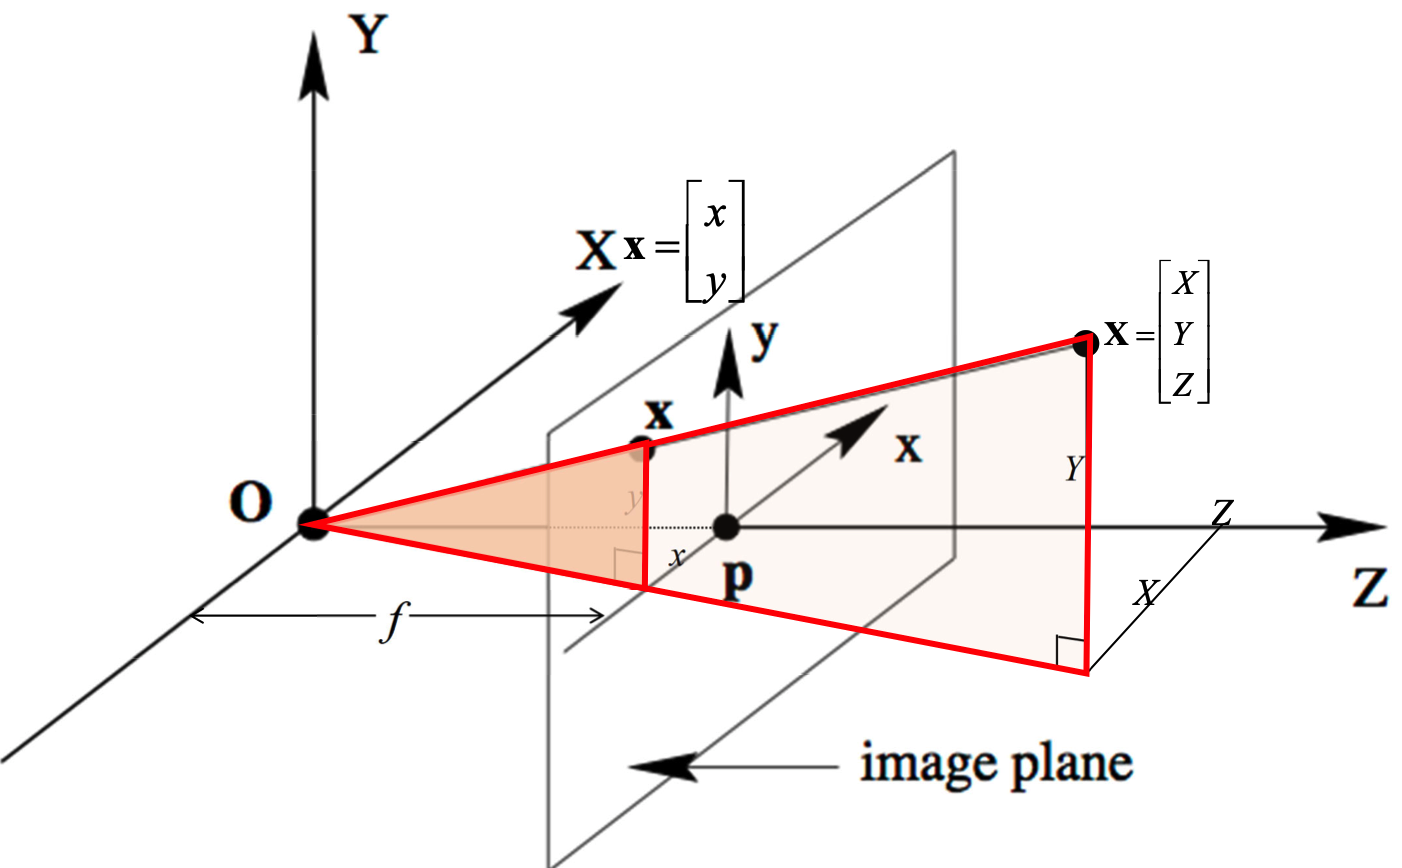
\includegraphics[width=1\textwidth]{./img/sy1.png} 
        \end{minipage}
    }
    \subfigure[相似三角形2]{
        \begin{minipage}[b]{0.45\textwidth}
        \centering
        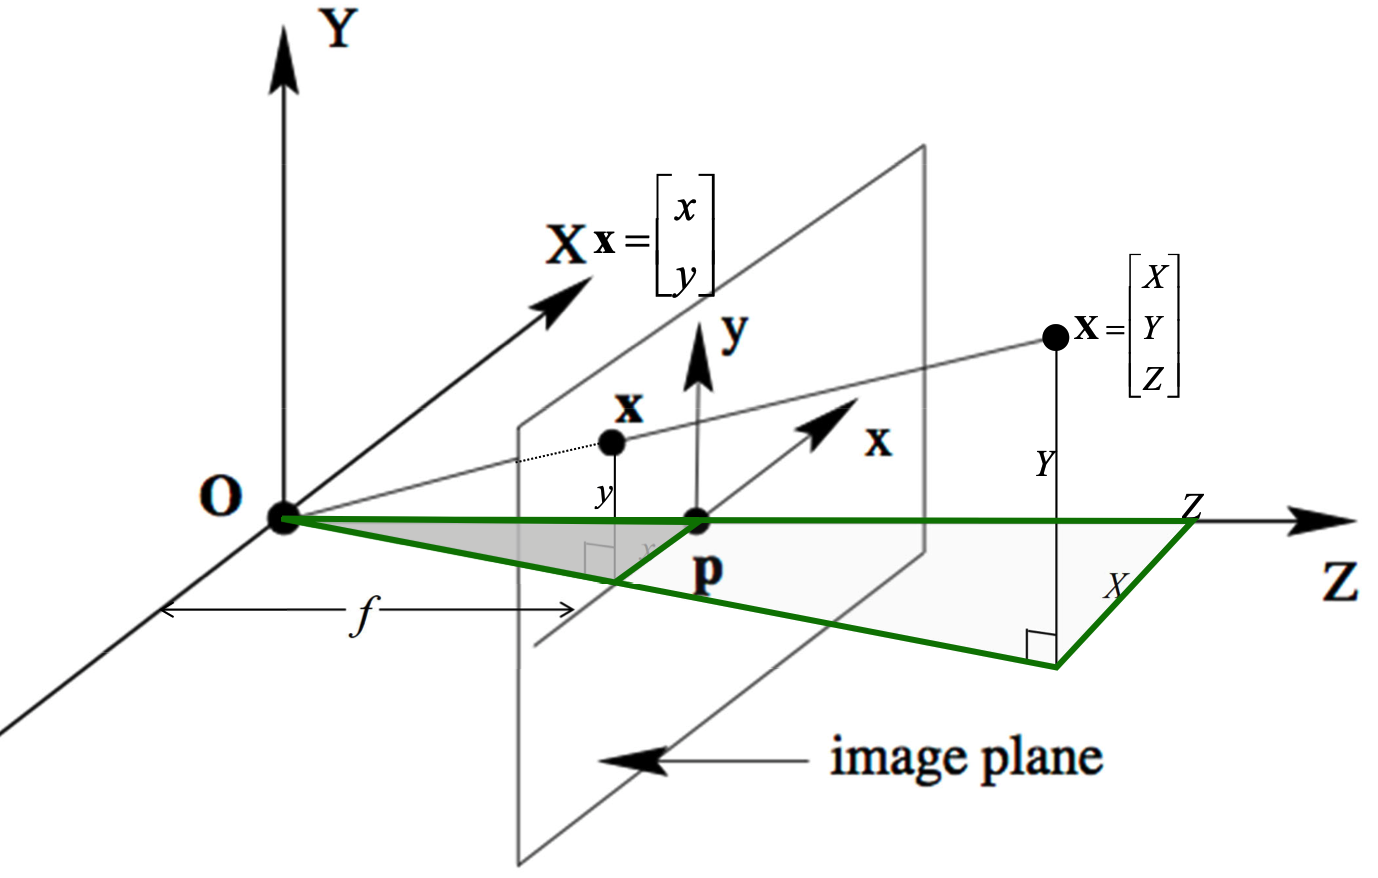
\includegraphics[width=1\textwidth]{./img/sy2.png}
        \end{minipage}
    }
    \caption{射影空间和欧式空间关系说明}
    \label{fig:sy}
\end{figure}

其中$\lambda$就是尺度变换因子。当$\lambda$变换的时候,描述的都是该像素点对应的三维空间直线上的所有点。
所以$\lambda$的变化并不影响「像素点和三维直线的关系」,所以我们将上公式简化为:
\begin{equation}
    \lambda\left[\begin{array}{l}
        x \\
        y \\
        f
        \end{array}\right]=\lambda f\left[\begin{array}{l}
        \frac{x}{f} \\
        \frac{y}{f} \\
        1
        \end{array}\right]=\lambda_{new}\left[\begin{array}{l}
        x_{new} \\
        y_{new} \\
        1
        \end{array}\right]
\end{equation}

此时的$[x_{new},y_{new}]^T$可以看作焦距为1时的图像平面上的点,但是我们将它齐次化之后,得到了$[x_{new},y_{new},1]^T$,他就有了新的含义,
在这里我把它理解为二维射影空间里的点。在这里我们可以看出,二维射影空间乘以一个尺度变换因子$\lambda_{new}$就可以表示出三维欧式空间(过原点)的一条直线,
即把二维平面和三维空间联系在了一起。(换一个角度思考,三维空间过原点的一条直线可以用三个参数来描述这个直线,也就是$\lambda_{new},x_{new},y_{new}$).

其实这种表示方法还不止可以表示出三维欧式空间过原点的所有直线,它还可以表示出三维欧式空间的无穷远点的集合(将它定义成一个球面).
这种表示方法为:
\begin{equation}
    \lambda\left[\begin{array}{l}
        x \\
        y \\
        f
        \end{array}\right]=\lim_{F \to +\infty}\lambda F\left[\begin{array}{l}
        \frac{x}{F} \\
        \frac{y}{F} \\
        \frac{f}{F}
        \end{array}\right]=\lambda_{new}\left[\begin{array}{l}
        x_{new} \\
        y_{new} \\
        0
        \end{array}\right]
\end{equation}

至于为啥要这么定义和表示,这样可以满足很多数学性质,以及很好的处理显示生活中平行但是图像上不平行的两条直线(例如消失在视野中的两条铁轨)。
具体的性质可以见https://blog.csdn.net/frozenspring/article/details/76034356?spm=1001.2014.3001.5501。

综上所述,我们可以得到最一般的射影空间(可理解为焦距为1情况下)表述如下(把$\lambda$去掉是因为等式左右两边在相差一个尺度因子的情况下是等价的):
\begin{equation}
    \left[\begin{array}{l}
        x \\
        y \\
        1
        \end{array}\right]\overset{\lambda}{=}\left[\begin{array}{l}
        X \\
        Y \\
        Z
        \end{array}\right]
    \label{eq:sy1}
\end{equation}

\begin{equation}
    \left[\begin{array}{l}
        x \\
        y \\
        0
        \end{array}\right]\overset{\lambda}{=}\left[\begin{array}{l}
        \infty \\
        \infty \\
        \infty
        \end{array}\right]
    \label{eq:sy2}
\end{equation}

\newpage
\subsection{相机模型}
描述相机的内外参数,内指的是焦距等参数,描述的是以相机为原点看世界;外指的是从相机原点到世界原点的旋转和平移关系。

最终得到的点就是二维像素点和世界三维欧式坐标点的关系,所以要借助上面的射影空间。

\subsubsection{相机内参数}
上面\ref{eq:sy1},\ref{eq:sy2}描述的是最一般射影空间(焦距为1),在实际的相机模型描述中,我们还保留焦距为$f$的射影空间表示方法:
\begin{equation}
    \label{eq:nc_basic}
    \left[\begin{array}{l}
        x \\
        y \\
        f
        \end{array}\right]=\lambda\left[\begin{array}{l}
            X_{cam} \\
            Y_{cam} \\
            Z_{cam}
            \end{array}\right]
        \overset{\lambda}{=}\left[\begin{array}{l}
        X_{cam} \\
        Y_{cam} \\
        Z_{cam}
        \end{array}\right]
\end{equation}
因为$f$是个未知数,所以我们要把他从变量中提取出来:
\begin{equation}
    \left[\begin{array}{l}
        x \\
        y \\
        1
        \end{array}\right]\overset{\lambda}{=}
        \left[\begin{array}{lll}
            1 &  & \\
              & 1 &\\
              &   & \frac{1}{f}
        \end{array}\right]
        \left[\begin{array}{l}
        X_{cam} \\
        Y_{cam} \\
        Z_{cam}
        \end{array}\right]\overset{\lambda}{=}
    \left[\begin{array}{lll}
        f &  & \\
          & f &\\
          &   & 1
    \end{array}\right]
    \left[\begin{array}{l}
    X_{cam} \\
    Y_{cam} \\
    Z_{cam}
    \end{array}\right]\overset{\lambda}{=}\mathbf{K}\left[\begin{array}{l}
        X_{cam} \\
        Y_{cam} \\
        Z_{cam}
        \end{array}\right]
    \label{eq:nc}
\end{equation}

其中的
$\left[\begin{array}{lll}
    f &  & \\
      & f &\\
      &   & 1
\end{array}\right]$就是相机的内参数,记作$\mathbf{K}$,$f$的单位应该是像素(焦距物理尺寸/单个CCD感光元宽度),当然这是理想情况下的。实际情况下考虑到感光元不是个标准的正方形($f_x, f_y$代表长宽,$s$)代表夹角,并且
图像的中心不是在CCD的中心而是在左上角($p_x. p_y$),真实的内参是:$\left[\begin{array}{lll}
    f_X & s  & p_x \\
      & f_y & p_y\\
      &   & 1
\end{array}\right]$

\begin{figure}[ht]
    \centering
    \subfigure[内参$f_x,f_y,s$]{
        \begin{minipage}[b]{0.45\textwidth}
        \centering
        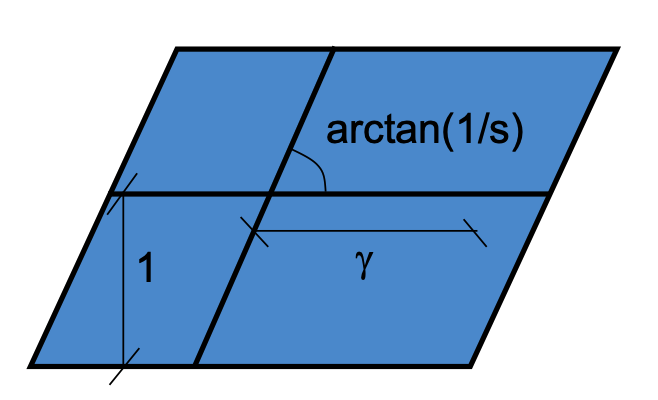
\includegraphics[width=1\textwidth]{./img/nc1.png} 
        \end{minipage}
    }
    \subfigure[内参$p_x,p_y$]{
        \begin{minipage}[b]{0.45\textwidth}
        \centering
        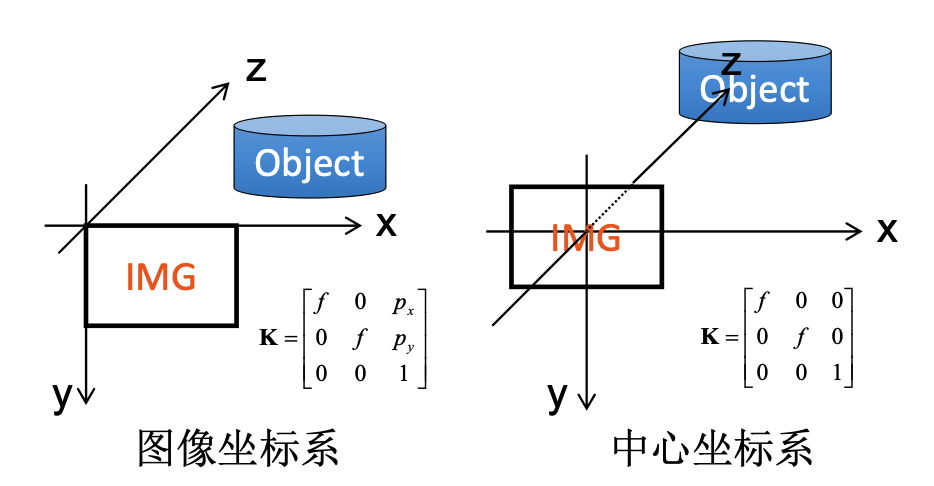
\includegraphics[width=1\textwidth]{./img/nc2.png}
        \end{minipage}
    }
    \caption{相机内参数示意图}
    \label{fig:nc}
\end{figure}

\subsubsection{相机外参数}
上面描述的是像素点到相机坐标系下的三维坐标点的关系,但是在真实世界中我们需要知道像素点和世界坐标系下三维坐标的关系,
相机外参数就是来描述相机坐标系到世界坐标系的转换关系。

这个就更简单了,因为两个三维坐标系的转换只涉及到旋转和平移(涉及到平移所以要先齐次化),
\begin{equation}
    \left[\begin{array}{l}
        X_{cam} \\
        Y_{cam} \\
        Z_{cam} \\
        1
        \end{array}\right]\overset{\lambda}{=}\left[\begin{array}{ll}
        \mathbf{R} & \mathbf{t} \\
        \mathbf{0}^{T} & 1
        \end{array}\right]\left[\begin{array}{c}
        X_{world} \\
        Y_{world} \\
        Z_{world} \\
        1
        \end{array}\right]
\end{equation}

那么这个外参数矩阵与上面公式中的旋转矩阵$\mathbf{R}$和平移向量$\mathbf{t}$有关。

\subsubsection{总结}
综上所述,想要把齐次化像素点(三维)和齐次化的世界坐标(四维)联系起来,还需要一个$3\times 4$的转换矩阵,表述如下:
\begin{equation}
    \left[\begin{array}{l}
        x \\
        y \\
        1
        \end{array}\right]\overset{\lambda}{=}\left[\begin{array}{lll}
        f & 0 & 0 \\
        0 & f & 0 \\
        0 & 0 & 1
        \end{array}\right]\left[\begin{array}{llll}
        1 & 0 & 0 & 0 \\
        0 & 1 & 0 & 0 \\
        0 & 0 & 1 & 0
        \end{array}\right]\left[\begin{array}{cc}
        \mathbf{R} & \mathbf{t} \\
        \mathbf{0}^{T} & 1
        \end{array}\right]\left[\begin{array}{c}
        X_{world} \\
        Y_{world} \\
        Z_{world} \\
        1
        \end{array}\right]
\end{equation}

简化如下:
\begin{equation}
    \label{eq:xjmx}
    \left[
        \begin{array}{l}
            x \\
            y \\
            1
        \end{array}
    \right]\overset{\lambda}{=}
    \mathbf{K}\left[\mathbf{R|\mathbf{t}}\right]\left[
        \begin{array}{l}
            X_{world} \\
            Y_{world} \\
            Z_{world} \\
            1
        \end{array}
    \right]
\end{equation}

其中$\mathbf{K}$是相机内参矩阵$\left[\begin{array}{lll}
    f &&\\
    &f&\\
    &&1
\end{array}\right]$

上述公式都是$\overset{\lambda}{=}$(差一个尺度因子时等价),但是这是简化在焦距$f=1$的2维平面上的,实际上在使用的时候,
例如我们想把3维点投射到2维焦距为$f$的图像平面上,我们就不能在$\overset{\lambda}{=}$上讨论了,要严格相等才行。

回忆公式\ref{eq:nc_basic}:
\begin{equation}
    \nonumber
    \left[\begin{array}{l}
        x \\
        y \\
        f
        \end{array}\right]=\lambda\left[\begin{array}{l}
            X_{cam} \\
            Y_{cam} \\
            Z_{cam}
            \end{array}\right]
        \overset{\lambda}{=}\left[\begin{array}{l}
        X_{cam} \\
        Y_{cam} \\
        Z_{cam}
        \end{array}\right]
\end{equation}

即$\lambda=\frac{f}{Z_{cam}}$,将$\lambda$带入公式\ref{eq:xjmx},又考虑到公式\ref{eq:nc}的第二个$\overset{\lambda}{=}$,
已经乘以过一次$f$,所以最终$\lambda=\frac{1}{Z_{cam}}$,最终得到严格相等的相机模型:
\begin{equation}
    \left[
        \begin{array}{l}
            x \\
            y \\
            1
        \end{array}
    \right]\overset{\lambda}{=}
    \mathbf{K}\left[\mathbf{R|\mathbf{t}}\right]\left[
        \begin{array}{l}
            X_{world} \\
            Y_{world} \\
            Z_{world} \\
            1
        \end{array}
    \right]=\frac{1}{Z_{cam}}
    \mathbf{K}\left[\mathbf{R|\mathbf{t}}\right]\left[
        \begin{array}{l}
            X_{world} \\
            Y_{world} \\
            Z_{world} \\
            1
        \end{array}
    \right]
\end{equation}

\newpage
\subsection{多视几何}
多视几何表述的就是从不同位置去拍摄同一个东西,相当于同一世界坐标系下的物体在不同的照片上有不同的像素位置,根据这些对应关系,我们可以构造线性方程求解相机的内外参数矩阵,
甚至是物体在世界坐标系下的坐标。
\begin{figure}[ht]
    \centering
    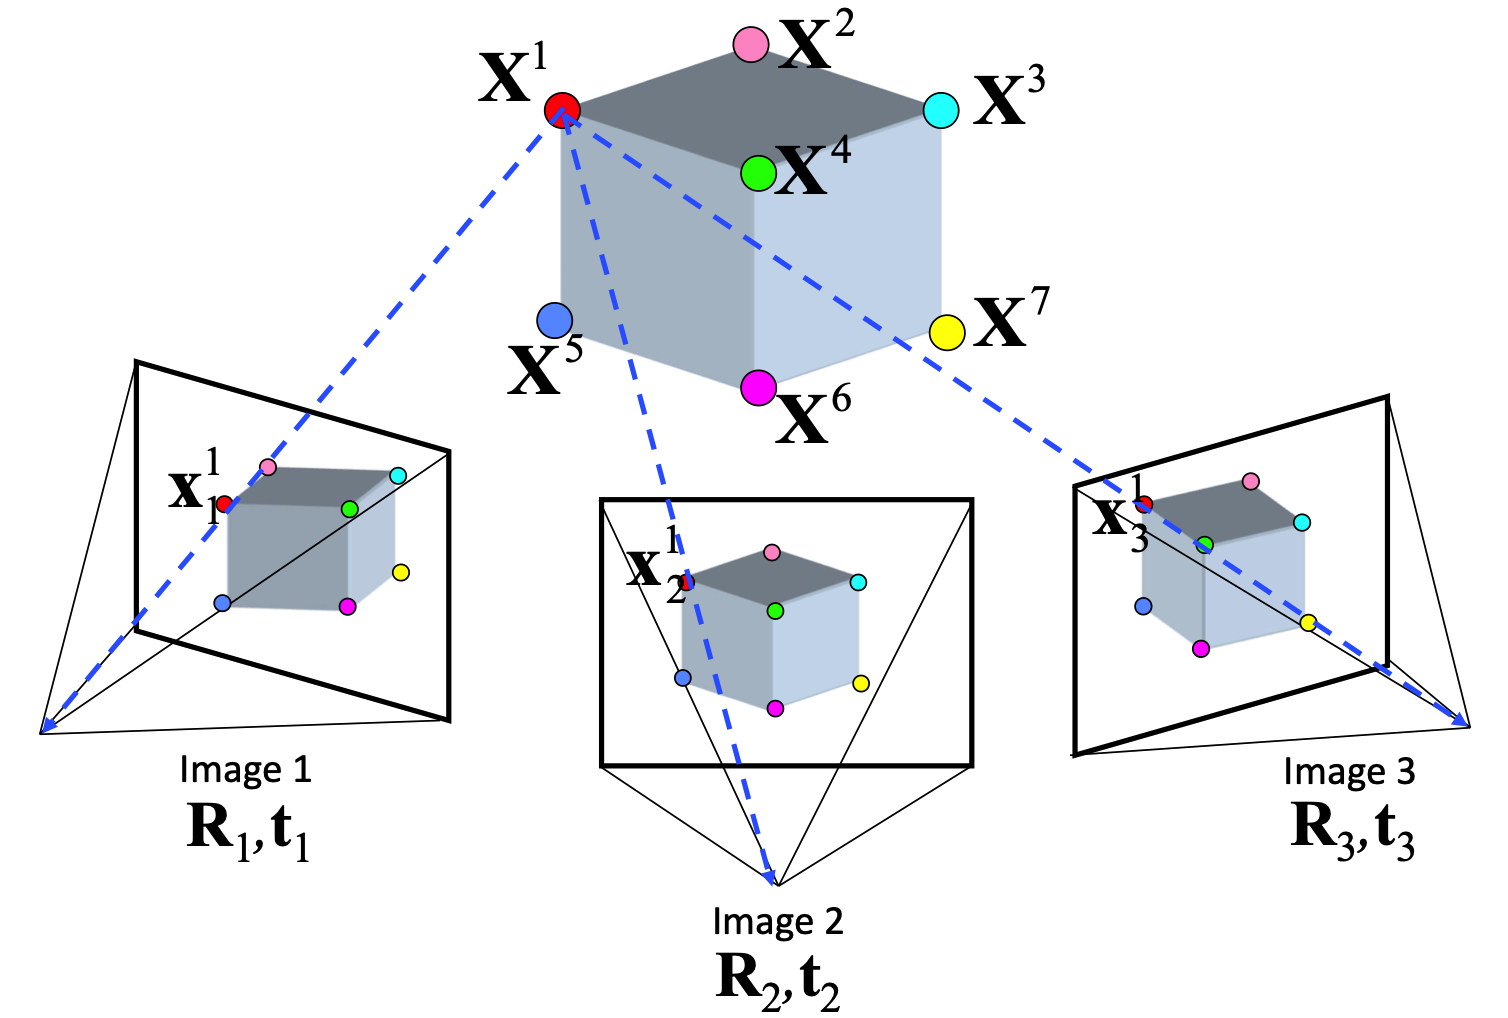
\includegraphics[scale=0.4]{./img/ds.png}
    \caption{多视几何}
    \label{fig:ds}
\end{figure}

\subsubsection{两视图几何--基本矩阵和本质矩阵}
多视角有点复杂,我们先从两视图来分析。这个基本矩阵呢,描述的就是两幅图像上“对应点像素位置”的关系。本质矩阵呢,就是描述两幅图像上“对应点的相机坐标系下的三维坐标”的关系。
这俩玩意其实道理是一样的,不过不同的地方用不同的表述方法可能方便点。

\begin{figure}[ht]
    \centering
    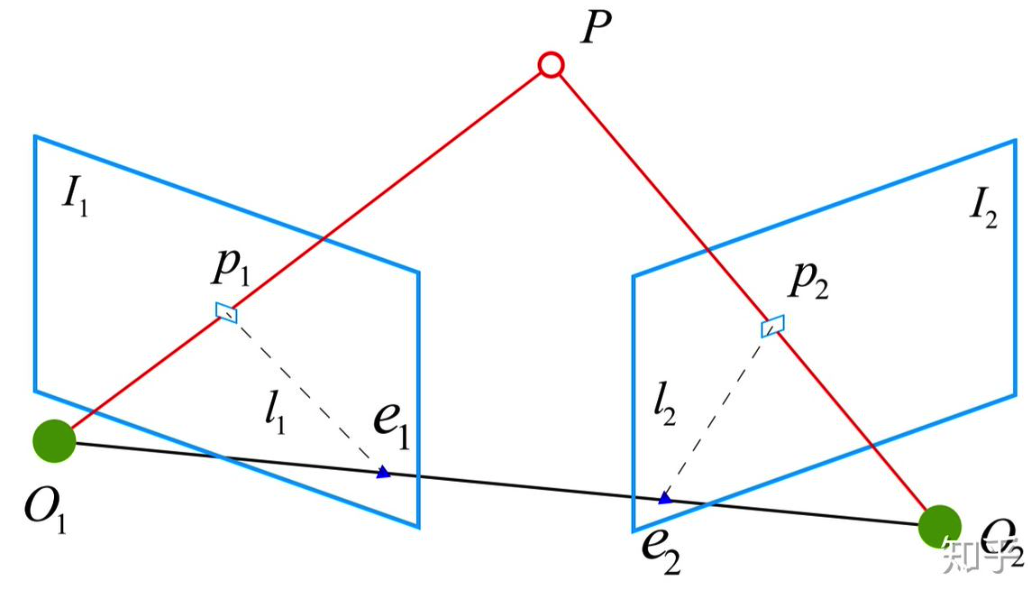
\includegraphics[scale=0.4]{./img/epipolar.png}
    \caption{两视图对极几何}
    \label{fig:ep}
\end{figure}

如图\ref{fig:ep}所示,$PO_1O_2$是极平面;$O_1O_2$是基线;$e_1$和$e_2$是对极点;$p_1e_1$和$p_2e_2$是对极线。

想要求得我们开始说的点的关系,就要用到$O_1P,O_1O_2,O_2P$在同一个平面上这个关系。即三个向量的叉乘为0.即
$O_1P\cdot (O_1O_2\times O_2P)=0$

那么$O_1P,O_1O_2,O_2P$分别是什么呢?我们可以分析一下:假设$P$在$O_1$为原点的相机坐标系下点坐标是$\mathbf{X_1}$,
在$O_2$为原点的相机坐标系下点坐标是$\mathbf{X_2}$,且$O_1$坐标系和$O_2$的关系是:$O_1$先平移$\mathbf{t}$,然后再逆时针旋转$\theta$矩阵$\mathbf{R}=\left[
    \begin{array}{ll}
        cos(\theta) & sin(-\theta)\\
        sin(\theta) & cos(\theta)
    \end{array}
\right]$,
那么点$\mathbf{X_1}$和点$\mathbf{X_2}$的关系是:$\mathbf{X_2}$先旋转$\mathbf{R}$,在平移$\mathbf{t}$得$\mathbf{X_1}$
(坐标系的变化和坐标点的变化是反过来的,见附录推导)。所以$\mathbf{X_1}=\mathbf{RX_2}+\mathbf{t}$.

以$O_1$为原点建立相机坐标系,我们可以得到:

$O_1O_2=\mathbf{t}$,

$O_1P=\mathbf{X_1}$,

$O_2P=\mathbf{X_1-t=RX_2}$.

进一步计算$O_1P\cdot (O_1O_2\times O_2P)=0$,有:$\mathbf{X_1}^T(\mathbf{t\times RX_2})=0$,这个叉乘我们可以表示成矩阵的形式(转换关系见附录):
\begin{equation}
    \mathbf{X_1}^T(\mathbf{[t]}_\times\mathbf{R)X_2}=0
\end{equation}

这里的$\mathbf{[t]}_\times\mathbf{R}$就是本质矩阵$\mathbf{E}$啦!!!!描述的是两个相机坐标系下P点坐标的转换关系。

下面的基本矩阵是一个道理,不过描述的是两张图片上像素位置($p_1$和$p_2$)的转换关系.根据公式\ref{eq:nc}:$\mathbf{x}\overset{\lambda}{=}\mathbf{KX}$,
有:
\begin{equation}
    \mathbf{x_1}^T(\mathbf{K_1}^{-T}[\mathbf{t}]_\times \mathbf{RK_2}^{-1})\mathbf{X_2}=0
\end{equation}
其中$\mathbf{K_1}^{-T}[\mathbf{t}]_\times \mathbf{RK_2}^{-1}$就是基础矩阵$\mathbf{F}$.

\subsubsection{两视图几何--8点法}
根据基础矩阵$F$和给定两视图中的对应点$x,x'$,我们有$\mathbf{x}^{\prime \mathrm{T}} \mathbf{F} \mathbf{x}=0$,按我们的第一印象,
矩阵含有两个内参矩阵(10DoF),一个旋转矩阵(3DoF),一个平移矩阵(3DoF),一共有16个未知数,但是要知道这些未知数不是独立的,
我们展开$\mathbf{x}^{\prime \mathrm{T}} \mathbf{F} \mathbf{x}=0$可以得到:
\begin{equation}
    \left[x_{1} x_{2}, x_{1} y_{2}, x_{1}, y_{1} x_{2}, y_{1} y_{2}, y_{1}, x_{2}, y_{2}, 1\right]\left[\begin{array}{c}
        f_{11} \\
        f_{12} \\
        f_{13} \\
        f_{21} \\
        f_{22} \\
        f_{23} \\
        f_{31} \\
        f_{32} \\
        f_{33}
        \end{array}\right]=0
\end{equation}
所以实际的未知参数是9,但是最后一个维度的变量是1,所以实际未知参数是8个,即8个方程求解:

\begin{equation}
    \left[\begin{array}{ccccccccc}
        x_{1}^{1} x_{2}^{1} & x_{1}^{1} y_{2}^{1} & x_{1}^{1} & y_{1}^{1} x_{2}^{1} & y_{1}^{1} y_{2}^{1} & y_{1}^{1} & x_{2}^{1} & y_{2}^{1} & 1 \\
        x_{1}^{2} x_{2}^{2} & x_{1}^{2} y_{2}^{2} & x_{1}^{2} & y_{1}^{2} x_{2}^{2} & y_{1}^{2} y_{2}^{2} & y_{1}^{2} & x_{2}^{2} & y_{2}^{2} & 1 \\
        x_{1}^{3} x_{2}^{3} & x_{1}^{3} y_{2}^{3} & x_{1}^{3} & y_{1}^{3} x_{2}^{3} & y_{1}^{3} y_{2}^{3} & y_{1}^{3} & x_{2}^{3} & y_{2}^{3} & 1 \\
        x_{1}^{4} x_{2}^{4} & x_{1}^{4} y_{2}^{4} & x_{1}^{4} & y_{1}^{4} x_{2}^{4} & y_{1}^{4} y_{2}^{4} & y_{1}^{4} & x_{2}^{4} & y_{2}^{4} & 1 \\
        x_{1}^{5} x_{2}^{5} & x_{1}^{5} y_{2}^{5} & x_{1}^{5} & y_{1}^{5} x_{2}^{5} & y_{1}^{5} y_{2}^{5} & y_{1}^{5} & x_{2}^{5} & y_{2}^{5} & 1 \\
        x_{1}^{6} x_{2}^{6} & x_{1}^{6} y_{2}^{6} & x_{1}^{6} & y_{1}^{6} x_{2}^{6} & y_{1}^{6} y_{2}^{6} & y_{1}^{6} & x_{2}^{6} & y_{2}^{6} & 1 \\
        x_{1}^{7} x_{2}^{7} & x_{1}^{7} y_{2}^{7} & x_{1}^{7} & y_{1}^{7} x_{2}^{7} & y_{1}^{7} y_{2}^{7} & y_{1}^{7} & x_{2}^{7} & y_{2}^{7} & 1 \\
        x_{1}^{8} x_{2}^{8} & x_{1}^{8} y_{2}^{8} & x_{1}^{8} & y_{1}^{8} x_{2}^{8} & y_{1}^{8} y_{2}^{8} & y_{1}^{8} & x_{2}^{8} & y_{2}^{8} & 1
        \end{array}\right]\left[\begin{array}{c}
            f_{11} \\
            f_{12} \\
            f_{13} \\
            f_{21} \\
            f_{22} \\
            f_{23} \\
            f_{31} \\
            f_{32} \\
            f_{33}
            \end{array}\right]=0
\end{equation}

\newpage
\section{相机标定与稀疏重建}
首先说一下多视几何引发出来的几个问题,假设我得到了多视几何上$n$个点:
\begin{equation}
    \nonumber
    \begin{array}{l}
        \mathbf{x}_{1}=\mathbf{K}_{1}\left[\mathbf{R}_{1} \mid \mathbf{t}_{1}\right] \mathbf{X} \\
        \vdots \\
        \mathbf{x}_{n}=\mathbf{K}_{n}\left[\mathbf{R}_{n} \mid \mathbf{t}_{n}\right] \mathbf{X}
        \end{array}
\end{equation}
\begin{itemize}
    \item 三角化:已知$\mathbf{x,K,R,t}$,求$\mathbf{X}$
    \item 姿态估计:已知$\mathbf{x,X,K}$,求$\mathbf{R,t}$
    \item 相机标定:已知$\mathbf{x,X}$,求$\mathbf{K,R,t}$
    \item 稀疏重建:已知$\mathbf{x}$,求$\mathbf{K,R,t,X}$
\end{itemize}

他们的求解有共同之处,其实就是列出线性方程,求解位置参数(由上到下需要的方程数要变多),但是由于误差的存在肯定无解,只能用伪逆求解
线性方程,然后得到初始解后在逐步迭代优化这个解。

下面看看相机标定和稀疏重建这两个方面。

\subsection{相机标定}
下面就是最一般的情况$p_{ij}\in(3,4)$是未知的。也是我们要求解的。
\begin{equation}
    \nonumber
    \left[\begin{array}{l}
        x_{i} \\
        y_{i} \\
        1
        \end{array}\right]=\left[\begin{array}{llll}
        p_{11} & p_{12} & p_{13} & p_{14} \\
        p_{21} & p_{22} & p_{23} & p_{24} \\
        p_{31} & p_{32} & p_{33} & p_{34}
        \end{array}\right]\left[\begin{array}{l}
        X_{i} \\
        Y_{i} \\
        Z_{i} \\
        1
        \end{array}\right]
\end{equation}

\begin{figure}[ht]
    \centering
    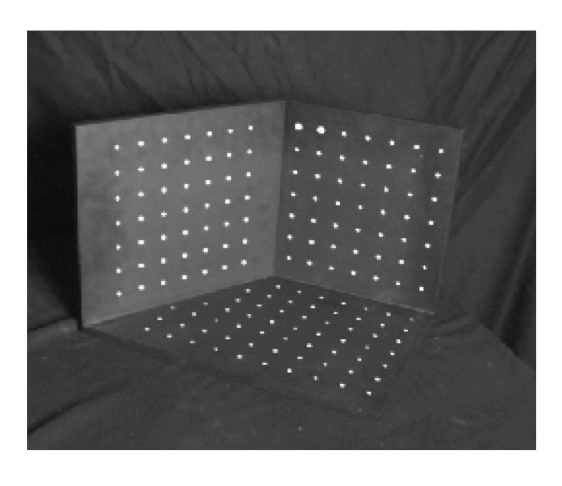
\includegraphics[scale=0.5]{./img/xjbd1.png}
    \caption{最一般的相机标定方式}
    \label{fig:xjbd1}
\end{figure}

我们将其展开,可以得到:
\begin{equation}
    \nonumber
    \left[\begin{array}{cccccccccccc}
        X_{i} & Y_{i} & Z_{i} & 1 & 0 & 0 & 0 & 0 & -x_{i} X_{i} & -x_{i} Y_{i} & -x_{i} Z_{i} & -x_{i} \\
        0 & 0 & 0 & 0 & X_{i} & Y_{i} & Z_{i} & 1 & -y_{i} X & -y_{i} Y & -y_{i} Z_{i} & -y_{i}
        \end{array}\right]\left[\begin{array}{c}
        p_{11} \\
        p_{12} \\
        p_{13} \\
        p_{14} \\
        p_{21} \\
        p_{22} \\
        p_{23} \\
        p_{24} \\
        p_{31} \\
        p_{32} \\
        p_{33} \\
        p_{34}
        \end{array}\right]=\left[\begin{array}{l}
        0 \\
        0
        \end{array}\right]
\end{equation}
即一共12个未知参数(11Dof「有时间在附录解释下」),但是一副对应点可以得到两个线性方程,所以最少只需要6个点得12个线性方程即可求解。但是这种方法是冗余的,我们可以参考下一种标定方法:

\begin{figure}[ht]
    \centering
    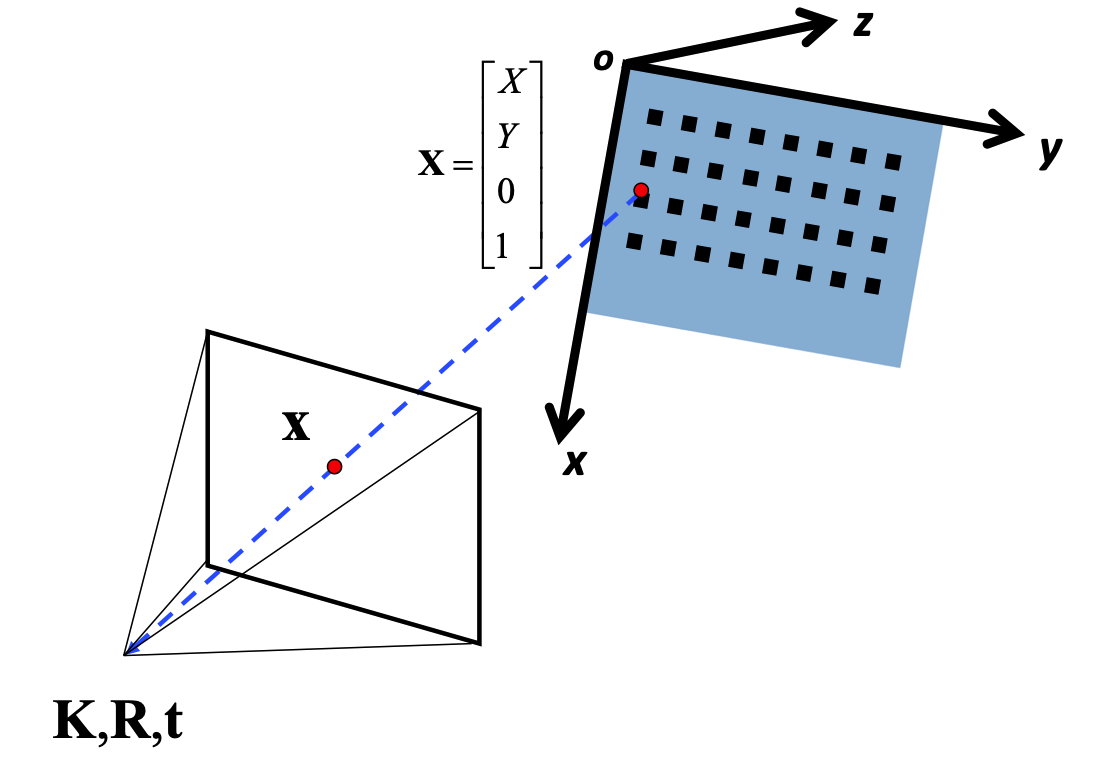
\includegraphics[scale=0.5]{./img/xjbd2.png}
    \caption{张友正标定法}
    \label{fig:xjbd2}
\end{figure}

通过限制三维世界坐标的$Z=0$,我们可以简化方程为:

\begin{equation}
    \nonumber
    \left[\begin{array}{l}
        x \\
        y \\
        1
        \end{array}\right]=\mathbf{K}[\mathbf{R} \mid \mathbf{t}]\left[\begin{array}{c}
        X \\
        Y \\
        0 \\
        1
        \end{array}\right]=
        \mathbf{K}\left[\begin{array}{llll}
        \mathbf{r}_{1} & \mathbf{r}_{2} & \mathbf{r}_{3}| & \mathbf{t}
        \end{array}\right]
        \left[\begin{array}{c}
        X \\
        Y \\
        0 \\
        1
        \end{array}\right]=
        \mathbf{K}\left[\begin{array}{lll}
        \mathbf{r}_{1} & \mathbf{r}_{2}| & \mathbf{t}
        \end{array}\right]
        \left[\begin{array}{c}
        X \\
        Y \\
        1
        \end{array}\right]
\end{equation}

其中$\mathbf{K}\left[\begin{array}{lll}
    \mathbf{r}_{1} & \mathbf{r}_{2}| & \mathbf{t}
    \end{array}\right]$为单应矩阵$\mathbf{H}\in(3,3)$(DOF=8),此时我们只需要4个对应点就得到8个方程就可以求解出相机参数。

到现在为止,我们求的是$\mathbf{H}$而不是相机内外参数$\mathbf{K,R,t}$,那么他们的转换关系是啥呢?

先把上述公式转换为:
\begin{equation}
    \label{eq:xjbd1}
    \left[\begin{array}{lll}
        \mathrm{r}_{1} & \mathrm{r}_{2} & \mid \mathbf{t}
        \end{array}\right]=\left[\begin{array}{lll}
        \mathbf{K}^{-1}\mathrm{h}_{1} & \mathbf{K}^{-1}\mathrm{~h}_{2} & \mathbf{K}^{-1}\mathrm{~h}_{3}
        \end{array}\right]
\end{equation}


再考虑到旋转向量的两个性质:
$\mathbf{r}_{1}^{T} \mathbf{r}_{2}=0 \quad\left\|\mathbf{r}_{1}\right\|=\left\|\mathbf{r}_{2}\right\|=1$

所以得到两个约束方程:
\begin{equation}
    \nonumber
    \begin{array}{c}
        \mathbf{h}_{1}^{T} \mathbf{K}^{-T} \mathbf{K}^{-1} \mathbf{h}_{2}=0 \\
        \mathbf{h}_{1}^{T} \mathbf{K}^{-T} \mathbf{K}^{-1} \mathbf{h}_{1}=\mathbf{h}_{2}^{T} \mathbf{K}^{-T} \mathbf{K}^{-1} \mathbf{h}_{2}
        \end{array}
\end{equation}

定义$\boldsymbol{\omega}=\mathbf{K}^{-T} \mathbf{K}^{-1}$,我们通过3组$h$即6个方程就可以求解出$\boldsymbol{\omega}$(因为$\mathbf{K}$的DoF=5),求出
$\boldsymbol{\omega}$后再正交分解(QR分解:正交+上三角)求出$\mathbf{K}$,然后根据公式\ref{eq:xjbd1}直接求解$r_1,r_2,t$,然后$r_3=r_1\times r_2$
\subsection{姿态估计}
PnP就是这个里面的问题,这里的n就是给定的匹配点的个数。然后再给定相机内参$\mathbf{K}$,要求外参数$\mathbf{R,t}$.
\begin{itemize}
    \item P2P:无穷多解;
    \item P3P:最多四个解,需要第4个点验证;
    \item P4P:最多四个解,当四点共面时有唯一解;
    \item P5P:最多两个解;
    \item EPnP:≥4组不共面点时有唯一解;
    \item PnP:线性求解(n>5).
\end{itemize}


\subsection{稀疏重建--BA--SFM}
我们回头看基本矩阵$\mathbf{x_1}^T\mathbf{Fx_2}=0$,仿佛就是来解决这个问题的,按照“两视图几何-8点法”可以解出$\mathbf{F}$,
不幸的是,$\mathbf{F}$无法唯一分解出$\mathbf{K_1,K_2,R,t}$.

但是我们放松一下条件,如果假设$\mathbf{K_1,K_2}$已知(这个也比较好获得,直接相机说明书等获得)。这样我们可以把目光投降本质矩阵
$\mathbf{X_1}^T\mathbf{EX_2}=0$.

那么我们可以先通过5点法求得$\mathbf{E}$,然后通过SVD分解求解$\mathbf{R,t}$。下面我们不加证明直接给出解:

假设相机1的$\mathbf{R_1=I,t_1=0}$,SVD分解得$\mathbf{E=U}diag(1,1,0)\mathbb{V}^T$。
此时相机2有4组解:
\begin{equation}
    \nonumber
    \begin{array}{l}
        {\left[\mathbf{R}_{2} \mid \mathbf{t}_{2}\right]=\left[\mathbf{U} \mathbf{W} \mathbf{V}^{T} \mid+\mathbf{u}_{3}\right]} \\
        {\left[\mathbf{R}_{2} \mid \mathbf{t}_{2}\right]=\left[\mathbf{U} \mathbf{W} \mathbf{V}^{T} \mid-\mathbf{u}_{3}\right]} \\
        {\left[\mathbf{R}_{2} \mid \mathbf{t}_{2}\right]=\left[\mathbf{U} \mathbf{W}^{T} \mathbf{V}^{T} \mid+\mathbf{u}_{3}\right]} \\
        {\left[\mathbf{R}_{2} \mid \mathbf{t}_{2}\right]=\left[\mathbf{U} \mathbf{W}^{T} \mathbf{V}^{T} \mid-\mathbf{u}_{3}\right]}
        \end{array}
\end{equation}

其中$\mathbf{W}=\left[\begin{array}{ccc}
    0 & -1 & 0 \\
    1 & 0 & 0 \\
    0 & 0 & 1
    \end{array}\right]$.

接下来怎么从这四个解中选一个呢?我们的原则是通过「三角化」求解$\mathbb{X}$,然后保留$\mathbb{X}$在相机前方最多的那个解。

\begin{figure}[ht]
    \centering
    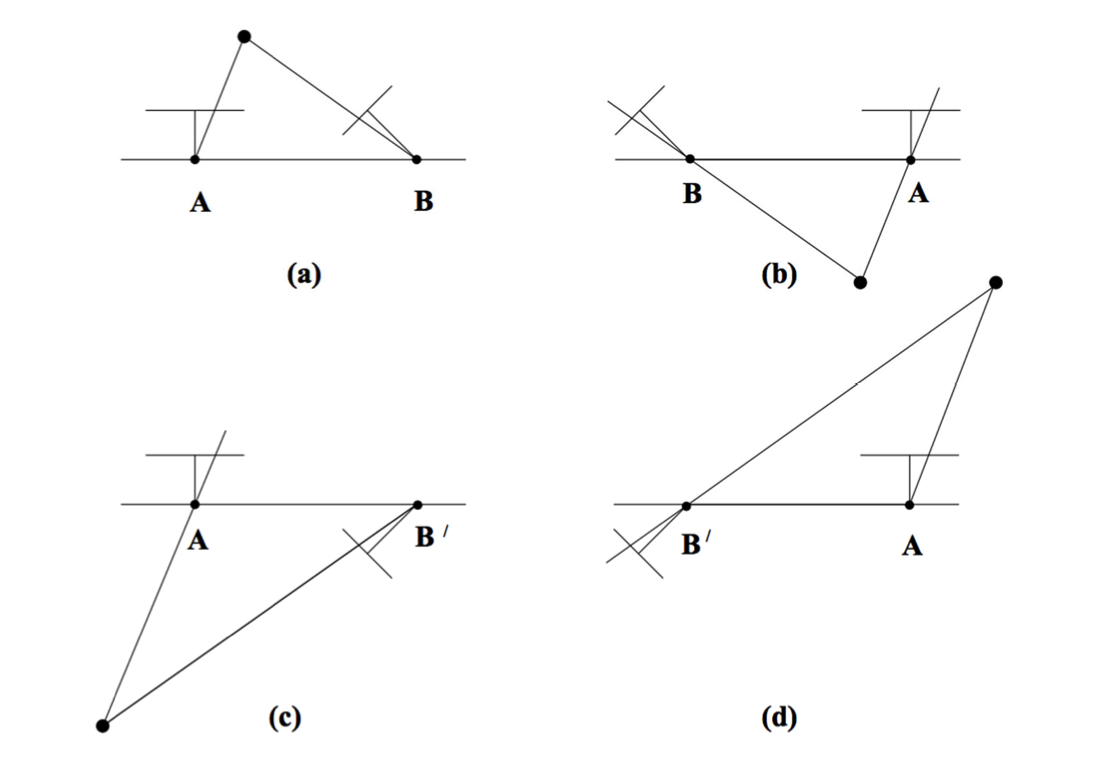
\includegraphics[scale=0.6]{./img/xscj1.png}
    \caption{稀疏重建解4选1}
    \label{fig:xscj1}
\end{figure}

这个可以当作初始解(代数误差最小),下面我们要迭代获得一个更精确的解。即求解重投影误差最小化(几何误差最小):

描述问题如下:在给定$\mathbf{K}$,通过对$\mathbf{E}$进行SVD分解后求得$\mathbf{R,t}$,并三角化得到$\mathbf{X}$,
迭代求解重投影误差最小化问题:
\begin{equation}
    \nonumber
    \min \sum_{i}\left\|\mathbf{P X}_{i}-\mathbf{x}_{i}\right\|^{2}
\end{equation}
最终得到几何误差最小化的$\mathbf{K,R,t,X}$.

如本节开头所说,其实三角化,相机标定,稀疏重建都可以先线性求一个初始解,然后在迭代求解重投影误差最小化,他们的异同如下图:

\begin{figure}[ht]
    \centering
    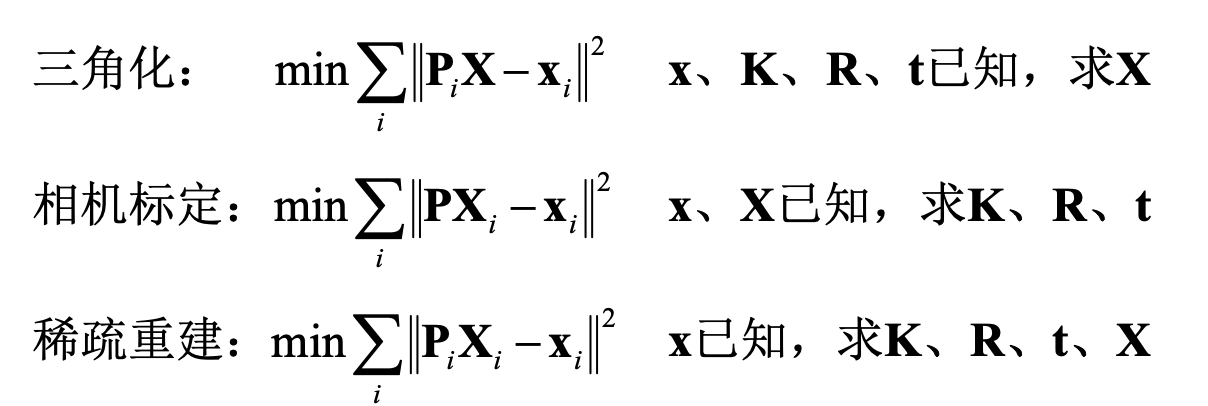
\includegraphics[scale=0.4]{./img/xscj2.png}
    \caption{重投影误差最小化}
    \label{fig:xscj2}
\end{figure}

下面长话短说,上面的$\mathbf{X}_i$在不同问题中含义不同,但是是$\mathbf{K,R,t,X}$的非线性组合,所以这可以看作非线性的最小二乘优化问题。
求解非线性最小二乘一般会用LM法(一种启发式的阻尼高斯牛顿法)。

所谓的BA:Bundle Adjustment 捆绑调整,说的就是用LM求解重投影误差最小化。

上面这一套稀疏重建从最小化代数误差然后再到BA优化得到最小化几何误差就是SFM(structure from motion)。一般比较好做的是二视图的SFM,增量式的SFM流程如下:
\begin{itemize}
    \item 选择初始图像对;
    \item 通过两视图SfM计算初始模型;
    \item 如果图像连接关系图还有未选择的图像\begin{itemize}
        \item 选择一幅能看到目前模型中最多3D点的图像;
        \item 根据3D‐2D点对应估计相机位姿;
        \item 三角化新的特征点Tracks
        \item bundle adjustment
    \end{itemize}
\end{itemize}

% --------------------------------------------------------------
%     You don't have to mess with an\Omega ything below this line.
% --------------------------------------------------------------

\newpage
\section{附录}
\subsection{坐标变换和坐标轴变换的关系}
如图\ref{fig:bh}所示:

$O_1$先向右上角平移一格,再逆时针旋转45度,得$O_2$,那么对于坐标系上的点来说,是相反的。

$P_2$先逆时针旋转45度,再右上移动一格,得$P_1$.证明如下:

\begin{equation}
    \nonumber
    P_1=\left[
        \begin{array}{l}
            2\\
            2\\
            1
        \end{array}
    \right]=
    \left[
        \begin{array}{lll}
            cos(45) & sin(-45) & 1\\
            sin(45) & cos(45) & 1 \\
            0  &  0  & 1
        \end{array}
    \right]
    \left[
        \begin{array}{l}
            \sqrt{2} \\
            0 \\
            1
        \end{array}
    \right]=
    \left[
        \begin{array}{lll}
            cos(\theta) & sin(-\theta) & t_x\\
            sin(\theta) & cos(\theta) & t_y \\
            0  &  0  & 1
        \end{array}
    \right]
    P_2
\end{equation}
\begin{figure}[ht]
    \centering
    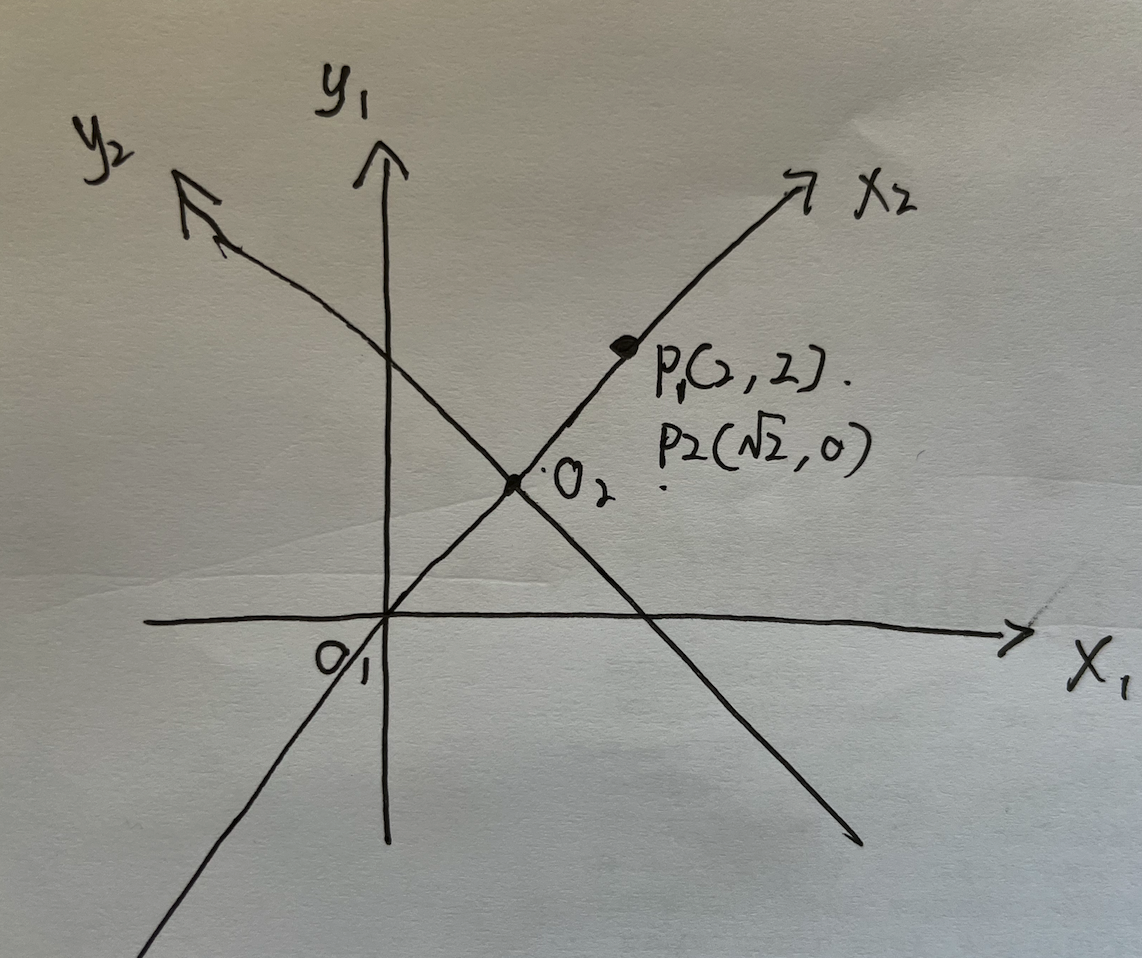
\includegraphics[scale=0.4]{./img/bianhuan.png}
    \caption{旋转平移变换}
    \label{fig:bh}
\end{figure}

\subsection{向量叉乘转矩阵形式}
两个向量如下:
\begin{equation}
    \nonumber
    \begin{array}{l}
        a=\left(a_{1}, a_{2}, a_{3}\right) \\
        b=\left(b_{1}, b_{2}, b_{3}\right)
        \end{array}
\end{equation}
通过引入单位向量,向量就可以转化为代数形式:
\begin{equation}
    \nonumber
    \begin{array}{l}
        a=a_{1} i+a_{2} j+a_{3} k \\
        \mathrm{~b}=\mathrm{b}_{1} i+b_{2} j+b_{3} k
        \end{array}
\end{equation}
定义单位向量间的运算规则
\begin{equation}
    \nonumber
    \begin{array}{ccc}
        i * i=0 & j * j=0 & k * k=0 \\
        i * j=k & j * k=i & k * i=j \\
        j * i=-k & k * j=-i & i * k=-j
        \end{array}
\end{equation}
计算叉乘:
\begin{equation}
    \nonumber
    \begin{array}{l}
        a \times b=\left(a_{1} i+a_{2} j+a_{3} k\right) *\left(b_{1} i+b_{2} j+b_{3} k\right) \\
        a \times b=\left(a_{2} b_{3}-a_{3} b_{2}\right) i+\left(a_{3} b_{1}-a_{1} b_{3}\right) j+\left(a_{1} b_{2}-a_{2} b_{1}\right) k
        \end{array}
\end{equation}
写成向量的形式:
\begin{equation}
    \nonumber
    a \times b=\left[\begin{array}{l}
        a_{2} b_{3}-a_{3} b_{2} \\
        a_{3} b_{1}-a_{1} b_{3} \\
        a_{1} b_{2}-a_{2} b_{1}
        \end{array}\right]
\end{equation}
变换得到叉乘矩阵:
\begin{equation}
    \nonumber
    a \times b=[a]_{\times} b=\left[\begin{array}{ccc}
        0 & -a_{3} & a_{2} \\
        a_{3} & 0 & -a_{1} \\
        -a_{2} & a_{1} & 0
        \end{array}\right]\left[\begin{array}{l}
        b_{1} \\
        b_{2} \\
        b_{3}
        \end{array}\right]
\end{equation}
\end{document}